\begin{defn}{Cone}
Let $\mathbf{a}_i\in\RR^m\setminus\vec{0}$ be the columns in some matrix 
$A\in \RR^{m \times n}$, and let $x_i\geq 0$ be the entries for some vector $\mathbf{x}\in \RR^n$.
 Then
\begin{equation*}
    V(A,\mathbf{x}) =\left \{ \sum_{i=1}^{n} x_i \mathbf{a}_i \right \},
\end{equation*}
is a cone. 
\end{defn}
In $\RR^2$ this reduces to a simple triangle, as seen in Figure~\ref{fig:cone_condition_true}
\begin{defn}{Cone Condition}~\label{def:cone_condition}
    Let $E$ be a Euclidean space and let $G$ be an open subset of $E$.
    Then $G$ fulfills the cone condition if
    \begin{equation*}
        \forall g \in G\,\, \exists x\in \RR^n
        \, \exists A\in \RR^{m \times n} \,\, :
        V(A,\mathbf{x})\neq \varnothing \land
        g + V(A, \mathbf{x}) \subset G. % + er translation
    \end{equation*}
    This means: at all points in $G$, we can create a non-empty cone,
     such that the cone is contained 
    in $G$.
\end{defn}

\begin{figure}[H]
    \centering
    \begin{subfigure}{.3\textwidth}
        \centering
        \begin{tikzpicture}
	\path[draw=black, line width =1pt, line join=round]  (0,0) .. controls (-0.2,1.5) .. (1,1)
		-- (1.5,1) .. controls (1,0) .. (1.2,-0.2)
		.. controls (1.5,-1.5) .. (-0.25,-1)
		.. controls (-0.5, -0.5) .. cycle;
  \node [isosceles triangle,
         isosceles triangle apex angle=20,
         rotate = 30,
         fill=gray!25,
         anchor=apex,
         minimum width=2pt] (t) at (1.5,1) {};    
\end{tikzpicture}
        \caption{Space which fulfill the Cone Condition}~\label{fig:cone_condition_true}
      \end{subfigure}
    \begin{subfigure}{.3\textwidth}
        \centering
        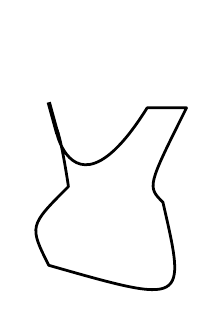
\begin{tikzpicture}
	\path[draw=black, line width =1pt, line join=round]  (0,0) .. controls (-0.3,2) and 
		(-0.25, -1) .. (1,1)
		-- (1.5,1) .. controls (1,0) .. (1.2,-0.2)
		.. controls (1.5,-1.5) .. (-0.25,-1)
		.. controls (-0.5, -0.5) .. cycle;
	\path[draw=black, line width = 1.5pt, line join=round] (-0.14,0.67) -- (-0.25,1.07);
\end{tikzpicture}
        \caption{Space which does not fulfill the Cone Condition}~\label{fig:cone_condition_false}
      \end{subfigure}
      \caption{The Cone Condition visualized}~\label{fig:cone_condition_visu}
\end{figure}
In Figure~\ref{fig:cone_condition_visu}, two spaces are visualized.
 The space in Figure~\ref{fig:cone_condition_true} fulfills the Cone Condition as seen 
 by the grey cone, which can be translated, rotated and scaled to any point, and still 
 be contained in the space. The space  
 in Figure~\ref{fig:cone_condition_false} does not fulfill the Cone Condition, as
in the upper left section of the space a cone cannot be drawn which is contained in the space.

